\documentclass[a4paper,12pt]{article}
\usepackage{tikz}
\usetikzlibrary{arrows,positioning}
\begin{document}

a. The idea behind \texttt{parallel-tree} is simple. Consider the list \texttt{(1 2 3)}. A balanced binary tree for this list should look like
\begin{center}
\begin{tikzpicture}
[level 2/.style={sibling distance=10mm}]
\node {\texttt{2}}
	child {node {\texttt{1}}}
	child {node {\texttt{3}}};
\end{tikzpicture}
\end{center}
The middle element from the list (2) becomes the root. Elements to the left of 2 (1) become go into the left subtree. Elements to the right of 2 (3) go into the right subtree. \\
In general for any given list the center element from the list becomes the root. Elements to the left of center go into the left subtree and elements to the right of centre go into the right subtree. This process can be applied recursively to contruct the complete tree. Keep in mind that for this to work the list must be ordered. This is exactly what \texttt{parallel-tree} does. It partitions the list into three parts as described. There is a recursive call to process elements to left of center. Then another recursive call to process elements to the right of center. Finally it constructs the tree with center element of the list as root and the left and right subtrees generated by the recursive calls.

\bigskip The tree produced by \texttt{list->tree} for the list \texttt{(1 3 5 7 9 11)}
\begin{center}
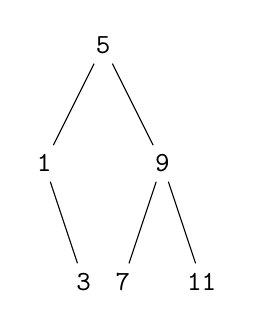
\begin{tikzpicture}
[level 2/.style={sibling distance=10mm}]
\node {\texttt{5}}
	child {node {\texttt{1}}
		child[missing] {node {}}
		child {node {\texttt{3}}}}
	child {node {\texttt{9}}
		child {node {\texttt{7}}}
		child {node {\texttt{11}}}};
\end{tikzpicture}
\end{center}

\bigskip b. The order of growth is $O(n)$ where is n is the number of elements in the list. This is because the procedure recurses for every single element of the list and each call of partial-tree takes contstant time (for all processing other than the recursive calls).

\end{document}